\chapter{Grundlagen}\label{kap:grundlagen}

%####################  CHAPTER 1: Grundlagen  #################

Dieses Kapitel beschreibt in den ersten Abschnitten die Grundlagen 
des Machine Learnings, und die Funktionsweise Künstlicher Neuronaler Netze,
insbesondere für Computer Vision Anwendungen.
Der letzte Abschnitt behandelt die für die Arbeit verwendete KI taugliche 
Hardware, den Neural Compute Stick 2.



%------------------- SECTION: Machine Learning ------------------

\section{Machine Learning}\label{sec:ml}

Beim Machine Lerining, welches ein Teilgebiet der Computerwissenschafen
ist, geht es um die Erstellung von Algorithmen, die Zusammenhänge in großen
Datenmengen erkennen, ohne explizit darauf programmiert worden zu sein.
Eine Form davon ist das \textit{Supervised Learning}, bei dem das Programm 
neben den Input Daten auch die Zugehörigen Ausgaben erhält um daraus 
Regeln für Zusammenhänge zwischen Ein- und Ausgabe Daten abzuleiten.

Dadurch unterscheidet sich das Vorgehen wesentlich zur klassischen Programmierung,
bei bei der die Regeln vorab definiert werden müssen.

\vspace{0.4cm}
\begin{center}
    
\tikzset{
    decision/.style={
        diamond,
        draw,
        text width=4em,
        text badly centered,
        inner sep=-1pt,
        node distance=8em
    },
    block/.style={
        rectangle,
        draw,
        text width=6em,
        %minimum widhth=6em,
        minimum height=3.5em,
        text centered,
        node distance=20em
    },
    arrow/.style={
        draw,
        >=latex,
        ->
    },
    textfeld/.style={
        %draw,
        text centered,
        node distance=1.5em
    }
}


\begin{tikzpicture}

    
    \node (system) [block] {Klassisches\\Programm};
    \node (system2) [block, right of=system] {ML\\Programm};

    \node [textfeld, left=of system.167] (inputs) {Daten};
    \node [textfeld, left=of system.193] (regeln) {Regeln};
    \node [textfeld, right=of system] (output) {Ausgaben};

    \node [textfeld, left=of system2.167] (inputs2) {Daten};
    \node [textfeld, left=of system2.193] (output2) {Ausgaben};
    \node [textfeld, right=of system2] (regeln2) {Regeln};
    
    \draw[arrow] (inputs) -- (system.167);
    \draw[arrow] (regeln) -- (system.193);
    \draw[arrow] (system) -- (output);
    
    \draw[arrow] (inputs2) -- (system2.167);
    \draw[arrow] (output2) -- (system2.193);
    \draw[arrow] (system2) -- (regeln2);
    

\end{tikzpicture}
    
\end{center}
\vspace{0.4cm}



Das ableiten der Regeln erfolgt beim Machine Learning in einem 
iterativen Prozess, welcher als Training bezeichnet wird.
Dabei werden die Zusammenhänge zwischen In- und Output Daten 
als mathematische Funktion betrachtet, welche numerisch 
angenähert wird.

Bei einem linearen Zusammenhang, handelt es sich
um eine Regression und bei einem kategorischen um 
eine Klassifizierung.

Weitere Formen neben dem \textit{Supervised Learning} sind das 
\textit{Unsupervised Learning}, bei der das Programm keine Labels 
erhällt, sondern diese selber finden 
soll, oder das \textit{Reinfocement Learning}, bei dem das Programm 
durch interaktion mit der Umwelt bestimmte aufgaben lernt.
Diese techniken wurden in der Bachelor Arbeit nicht verwendet 
und werden daher nicht näher erläutert.

%------------------- SECTION: Neuronale Netze -------------------

\subsection{Künstliche Neuronale Netze} \label{subsec:nn}

Für komplexe Input Daten, wie beispielsweise Bilder, bei denen 
die einzelnen Pixelwerte als Inputs und der Inhalt des Bildes als 
Output dienen, werden in der Regel künstliche Neuronale Netze verwendet.
Diese sind eine Form des Machine Learings und bestehen aus einer 
vielzahl an miteinander verbundener Neuronen. Durch unterschiedlich 
starke Gewichtungen der einzelnen Verbindungen, auch Gewichte genannt, 
können für unterschiedliche Input Daten die entsprechenden Outputs 
gefunden werden.

\begin{figure}[H]
    \centering
    \label{fig:nn}
    \def\svgwidth{0.65\columnwidth}
    \footnotesize
    \begin{neuralnetwork}[height=1]
    \newcommand{\nodetextclear}[2]{}
    \newcommand{\nodetexth}[2]{$h_#2$}
    \newcommand{\nodetextx}[2]{$x_#2$}
    \newcommand{\nodetexty}[2]{$y_#2$}
    \inputlayer[count=3, bias=false, title=Input\\layer, text=\nodetextx]
    \hiddenlayer[count=4, bias=false, title=Hidden\\layer, text=\nodetexth] \linklayers
    \outputlayer[count=2, title=Output\\layer, text=\nodetexty] \linklayers
\end{neuralnetwork}
\end{figure}

Die richtige gewichtung der Parameter erfolgt dabei in einem iterativen Trainingsprozess, 
welcher aus den drei schritten:


\begin{itemize}
    \item \textit{Forward Pass} anhand aktueller Gewichte vorhersage aus den Inputs treffen
    \item \textit{Fehlerbestimmung} Abweichung zum tatsächlichen werten berechnen
    \item \textit{Backpropagation} minimierung der Fehlerfunktion durch Anpassung der Gewichte
\end{itemize}

besthet und in Abbildung \ref{fig:train} schematisch dargestellt ist.



\begin{figure}[H]
    \centering
    \label{fig:train}
    
\tikzstyle{process} = [rectangle, fill=blue!20, minimum width=2.5cm, minimum height=1cm, text centered, draw=black]
\tikzstyle{arrow} = [thick,->,>=stealth]

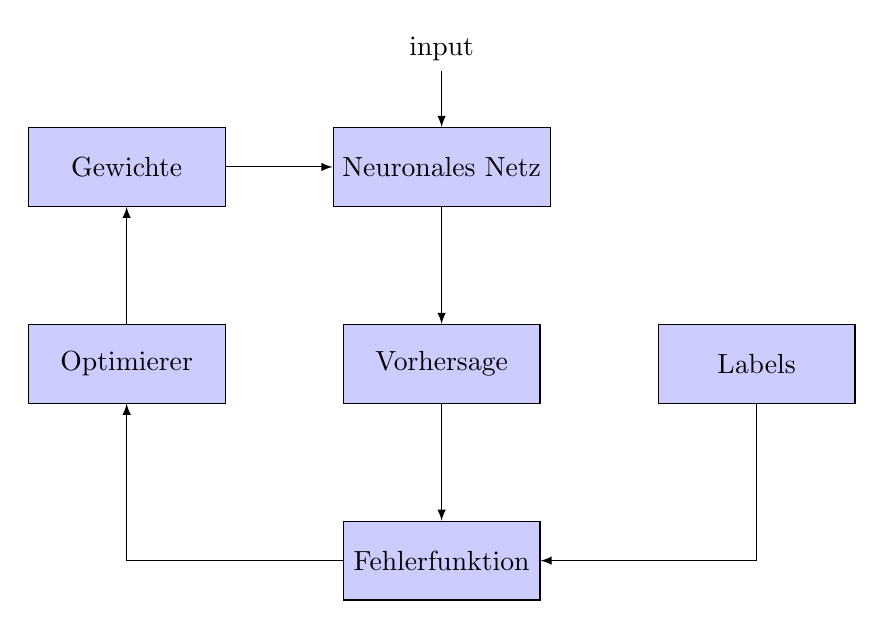
\begin{tikzpicture}[node distance=1.6cm]

  \begin{scope}[node distance=2.5cm]
    \node (nn)      [process]                   {Neuronales Netz};
    \node (pred)      [process, below of=nn]      {Vorhersage};
    \node (loss)      [process, below of=pred]      {Fehlerfunktion};
    
  \end{scope}
  
  \begin{scope}[node distance=4cm]
    \node (opt) [process, left of=pred]      {Optimierer};
    \node (weights)  [process, left of=nn] {Gewichte};
    \node (labels)   [process, right of=pred]  {Labels};
  \end{scope}

  \node (input) at (0,1.5) {input};

  \draw[arrow] (input) -- (nn);

  \draw[arrow] (nn) -- (pred);
  \draw[arrow] (pred) -- (loss);

  \draw[arrow] (labels) |- (loss);
  \draw[arrow] (loss) -| (opt);

  \draw[arrow] (opt) -- (weights);
  \draw[arrow] (weights) -- (nn);
  
    
\end{tikzpicture}

    \caption{Trainingsablauf NN}
\end{figure}




Durch merhfaches durchlaufen der Schritte wird die Fehlerfunktion soweit minimiert, 
sodass das Modell auch für neue Input Daten die richtigen Aussagen treffen kann.
Die mathematischen berechnungen der einzelnen Schritte werden im folgeden erläutert.


\subsubsection{Forward Pass}
Im \textit{Forward Pass} werden die Inputs durch alle Schichten hindurch 
gereicht, um in der letzten Schicht den gewünschten Output zu liefern.
Dabei erhält jedes Neuron die mit $w_{i}$ gewichteten Ausgabewerte aller
Neuronen der vorherigen Schicht und summiert diese zusammen mit einem konstanten 
Bias Wert $b$ auf. 
Mithilfe einer Aktivierungsfunktion wird der Wert auf einen bestimmenten Bereich 
skalliert \ref{fig:neuron}


\begin{figure}[H]
    \centering
    \label{fig:neuron}
    \begin{tikzpicture}[
    % define styles    
    init/.style={ 
         draw, 
         circle, 
         inner sep=2pt,
         font=\Huge,
         join = by -latex
    },
    squa_draw/.style={ 
        draw,
        font=\Large,
        join = by -latex
    },
    squa/.style={ 
        font=\Large,
        join = by -latex
    }
]
% Top chain x1 to w1
\begin{scope}[start chain=1]
    \node[on chain=1] at (0,1.5cm)  (x1) {$x_1$};
    \node[on chain=1,join=by o-latex] (w1) {$w_1$};
\end{scope}
% Middle chain x2 to output
\begin{scope}[start chain=2]
    \node[on chain=2] (x2) {$x_2$};
    \node[on chain=2,join=by o-latex] {$w_2$};
    \node[on chain=2,init] (sigma) {$\displaystyle\Sigma$};
    \node[on chain=2,squa_draw,label=below:{\parbox{2cm}{\centering Aktivierungs-funktion}}]   {$g(z)$};
    \node[on chain=2,squa,label=below:Output,join=by -latex] {$y_{out}$};
\end{scope}
% Bottom chain x3 to w3
\begin{scope}[start chain=3]
    \node[on chain=3,label=below:Inputs] at (0,-1.5cm) 
    (x3) {$x_3$};
    \node[on chain=3,label=below:Gewichte,join=by o-latex]
    (w3) {$w_3$};
\end{scope}
% Bias
\node[label=above:\parbox{2cm}{\centering Bias \\ $b$}] at (sigma|-w1) (b) {};
% Arrows joining w1, w3 and b to sigma
\draw[-latex] (w1) -- (sigma);
\draw[-latex] (w3) -- (sigma);
\draw[o-latex] (b) -- (sigma);

\end{tikzpicture}

% von https://medium.com/momenton/typesetting-neural-network-diagrams-with-tex-4920b6b9fc19
    \caption{Einzelnes Perzeptron}
\end{figure}


Um den Forward Pass für eine gesammte Schicht, bestehend aus 
einer Vielzahl an Neuronen, zu berechnen, werden die Schichten 
als Vektoren und die Gewichte als Matrizen dargestellt.

Die Matrixmultiplikation aus dem Vektor der vorherigen 
Schicht $x$ mit der Gecwichtsmatrix $W$ ergibt die Werte
des Vektors $z$ der aktuellen Schicht,

\begin{equation}
    \label{eq:forward}
    z = W^{T}x+b
\end{equation}

Dieser wird dann elementweise einer nichtlinearen Aktivierungsfunktion
$g(z)$ übergeben wird.

Für mittlere Schichten (Hidden Layer) wird dabei oft die in \ref{plot:relu} dargestellte
\textit{ReLU Funktion} verwendet welche positive Werte beibehällt und negative 
Werte zu 0 setzt.

Das hat den Vorteil, \dots

Um für die Outputs einen Wahrscheinlichkeits Wert zwischen 0 und 1 
zu erhalten, wird in der letzten Schicht für eine binäre Klassifikation 
die Sigmoid Funktion (\ref{plot:sidmoid}) verwendet,
welche S-Förmig zwischen 0 und 1 verläuft.

\vspace{1cm}

\begin{minipage}{0.5\textwidth}
    \centering
    \begin{equation*}
        \label{eq:relu}
        g(z) = max\{0,z\}
    \end{equation*}
\end{minipage}
\begin{minipage}{0.5\textwidth}
    \centering
    \begin{equation*}
        \label{eq:sidmoid}
        g(z) = \frac{1}{1 + e^{-x}}
    \end{equation*}    
\end{minipage}

\vspace{1cm}

\begin{minipage}{0.5\textwidth}
    \centering
    \label{plot:relu}
    \begin{tikzpicture}[scale=0.6]
    \begin{axis}
        %scale only axis=true,
        [
            scale only axis=true,
            width=0.8\textwidth,
            height=5cm,
            axis x line=middle,
            axis y line=center,
            tick align=outside
        ]
        
        \addplot
        [
            blue,
            mark=none,
            smooth,
            domain=-3:6
        ] 
        (x,{(x>=0)*x});

	\end{axis}
\end{tikzpicture}
    \captionof{figure}{ReLU Funktion} 
\end{minipage}
\begin{minipage}{0.5\textwidth}
    \centering
    \label{plot:sigmoid}
    \begin{tikzpicture}[scale=0.8]
    \begin{axis}
        %scale only axis=true,
        [
            scale only axis=true,
            width=\textwidth,
            height=5cm,
            % xmin=-6,
            % xmax=6,
            axis x line=middle,
            axis y line=center,
            tick align=outside
        ]
        
        \addplot
        [
            blue,
            mark=none,
            smooth,
            domain=-6:6
        ] 
        (x,{1/(1+exp(-x))});

	\end{axis}
\end{tikzpicture}
    \captionof{figure}{Sigmoid Funktion} 
\end{minipage}

\vspace{1cm}


Für eine Kategorische Ausgabe mit mehr als zwei Werten wird 
die Softmax (\ref{eq:softmax}) Funktion verwendet, welche eine Wahrscheinlichkeits 
Verteilung über alle Ausgebe Neuronen generiert.

\begin{equation}
    \label{eq:softmax}
    g(z) = \frac{e^{z}}{\sum e^{x}}
\end{equation}


\subsubsection{Fehlerbestimmung}
Die Abweichung des geschätzten Werts, welche an den Neuronen der letzen Schicht 
vorliegen, zum tatsächlichen Werten, dem Label, wird mithilfe einer geeigneten
Fehlerfunktion bestimmt. Für eine Lineare Regression wird dabei z.B. 
der absolute oder quadratischen Abstand verwendet.

Für Klassifikationsmodelle wird meistens eine logarithmische Fehlerberechnung, wie 
die \textit{Cross Enropy Funktion} \ref{eq:crossentropy} verwendet.

\begin{equation}
    \label{eq:crossentropy}
    L = \hat{y}log(y) + (1 - \hat{y})log(1 - y)
\end{equation}

Durch den Logarithmus wird der Loss um so größer, je weiter die Schätzung $y$ vom 
tatsächlichen Wert $\hat{y}$ abweicht.
%hier plot


\subsubsection{Backpropagation}

Durch Berechnung des Gradienten der Fehlerfunktion kann ermittelt 
werden in welche Richtung die Gewichte angepasst werden müssen,
sodass diese sich im nächsten Durchgang minimiert.

Dafür wird die die Fehlerfunktion $L$ für jede Schicht partiell nach den 
Gewichten $w$ abgeleitet, was wie in gl. \ref{eq:backprop} dargestellt mithilfe der 
Kettenregel über die Aktivierungsfunktion $z$ geschieht.


\begin{equation}
    \label{eq:backprop}
    \frac{\partial L}{\partial w} = \frac{\partial L}{\partial z}\frac{\partial z}{\partial w}
\end{equation}
Mit dem ermittelten Gradienten werden dann die Gewichte nach Gleichung \ref{eq:update_wieghts} angepasst.
\begin{equation}
    \label{eq:update_wieghts}
    w  \leftarrow w - \eta \frac{\partial L}{\partial w}
\end{equation}

wobei die \textit{Lernrate} $\eta$ die Schrittweite ist, mit der die
Anpassungen vorgenommen werden.





%------------------- SUBSECTION: Validierung -------------------
\subsection{Validierung und Overfitting}\label{subsec:validation}

Um überprüfen zu können, ob und wie gut ein Modell die Zusammenhänge
in den Trainingsdaten generalisiert hat, dh auch für neue Daten
anwendbar ist,
wird der Datensatz in einen Trainings- und einen Testdatensatz aufgeteilt.

Während des Trainings wird für beide Sätze der Fehler berechnet, 
die korrektur der Gewichte mittels Backpropagation erfolgt
jedoch nur anhand der Trainingsdaten.

Entsteht eine Abweichung der beiden Fehlerfunktion wie in 
\ref{fig:overfitting} dargestellt, findet eine Überanpassung 
(\textit{Overfitting}) des Modells an die Trainingsdaten statt.

\vspace{2cm}
\begin{figure}[H]
    \centering
    \def\svgwidth{0.5\textwidth}
    \input{Bilder/overfitting.pdf_tex}
    \caption{Overfitting, anhand der Losskurven}
    \label{fig:overfitting}
\end{figure}
% vorlage: https://de.m.wikipedia.org/wiki/Datei:Overfitting_svg.svg
% \cite{overfittingPlot}

Gründe dafür sind zu wenig Trainingsdaten oder ein zu komplexes Model, 
welches sich aufgrund der vielen Parameter wie bei eine Funktionen hohen
grades, die Möglichkeit hat sich an jeden Datenpunk 
anzupassen und damit nicht mehr generalisierbare Aussagen 
für neue Datenpunkte treffen kann.

\vspace{1cm}
\begin{figure}[H]
    \centering
    \def\svgwidth{0.95\textwidth}
    \input{Bilder/over_under_fit.pdf_tex}
    \caption{}
    \label{fig:over_under_fit}
\end{figure}
\vspace{1cm}


Stehen nicht mehr Trainingsdaten zur verfügung, kann Overfitting
mit einer der folgeden Techniken verhindert werden.


\subsubsection{Augmentierung}
Bei Augmentierung werden aus den vorhandenen Daten künstlich mehr 
Daten generiert, in dem an den Bildern geometrische transformationen 
oder manipulationen der pixelwerte vorgenommen werden.

\subsubsection{Regularisierung der Parameter (L1/L2)}
Bei Regularisierung wird der Lossfuction als weiterer Term
eine aufsummierung aller Gewichte hinzugefügt,
wodurch diese bei der Minimierung des Lossfunktion 
klein gehalten werden und damit einhergend weniger potential 
zum Overfitting besteht.

\begin{equation}
    \label{eq:regularization}
    J = L + \lambda \sum_{i} w_{i}^{2}
\end{equation}

\subsubsection{Dropout}
Beim Dropout werden in mit einer bestimmten Wahrscheinlichkeit 
einige Neuronen Neuronen (Bsp 50\%) zu 0 gesetzt, um 
alternative Gewichtsanpassungen zu erzwingen.

\begin{figure}[H]
    \centering
    \includegraphics[width=0.6\textwidth]{dropout.png}
    \caption{Dropout, Quelle: \cite{maksutovDeepStudyNot2018}}
    \label{fig:dropout}
\end{figure}

\subsubsection{Early Stopping}
Beim erly Stopping wird das Traing an der 
Stelle unterbroche, an der die Lossfunktion ihr 
Minimum erreicht hat, markierte stelle in 
\ref{fig:overfitting}.


%------------------- SUBSECTION: ML Frameworks ---------------
\subsection{Machine Learning Frameworks}

Machine Larning Algorithmen beeinhalten eine vielzahl an komplexen
Berechnungsschritten und Parametern. Um diese diese nicht jedesmal 
von Grund auf neu implementieren zu müssen bieten 
Frameworks eine vereinfachte Möglichkeit die Modelle zu konstruieren.

Einige der bekannten Open Source Frmaworks sind Tensorflow,
Caffe, Torch, Kaldi oder Scikit-Learn.

TensorFlow, welches in der Thesis verwendet wurde, stammt von 
Google und ist ein aufgrund seiner hohen Flexibilität besonders 
in der Forschung oft verwendetes Framework.





%---------------- SUBSECTION: Convolutional ----------------
\section{Convolutional Neural Networks}\label{subsec:cnn}

Convolutional Neural Networks (CNNs) erweitern 
die in Abschnitt \ref{subsec:nn} beschriebenen
\textit{Feed Forward Netze} um zusätzliche Schichten,
die vor der eigentliche klassifizierung ausgeführt werdem
und Merkmale aus den Input Daten herausextrahieren.

Diese Schichten enthalten den Input als zwei 
dimensionale Matrix und führen darauf eine 
mathematische Faltungsoperation aus.

CNNs kommen größtenteils in der Bilderkennung zum 
Einsatz, weitere Anwendungsgebiete sind 
die Spracherkennung.

Anstatt das alle Neuronen zweier benachbarter Schichten 
durch gewichtete Parameter miteinander verbunden sind, 
stellen kleinere, sogenannte Filter Matrizen, die 
Parameter dar.

Diese werden zeilenweise über das Input Bild 
geschoben, wobei an jeder Stelle eine mathematische 
Faltung mit dem überlappten Bereich des Input 
Bildes durchgeführt wird. Abbildung \ref{fig:faltung1}
und \ref{fig:faltung2} veranschaulichen diesen Vorgang.


\vspace{1cm}
\begin{minipage}{0.5\textwidth}
    \label{fig:faltung1}
    \centering
    \includegraphics[width=0.9\textwidth]{convolution.png}
    \captionof{figure}{Faltung, \cite{researcherSimpleIntroductionConvolutional2019}}
\end{minipage}
\begin{minipage}{0.5\textwidth}
    \label{fig:faltung2}
    \centering
    \includegraphics[width=0.9\textwidth]{convolution-layer-a.png}
\end{minipage}
\vspace{1cm}

Jedes Ergebniss einer Faltung ergibt einen Wert für 
die nächste Schicht, die dadurch 
ein Korellationsverhälltniss von zwischen
Filter Matrix und Input Bild erhält.

So werden in den Filtern definierte Muster, wie 
beispielsweise vertikale Linien, 
aus dem Inputbild herausextrahiert und in 
den Folgeschichten, als Feature Maps abgebildet.


\vspace{1cm}
\begin{equation}
    \label{eq:faltung}
    \begin{pmatrix}
        10 & 10 & 10 & 0 & 0 & 0\\
        10 & 10 & 10 & 0 & 0 & 0\\
        10 & 10 & 10 & 0 & 0 & 0\\
        10 & 10 & 10 & 0 & 0 & 0\\
        10 & 10 & 10 & 0 & 0 & 0\\
        10 & 10 & 10 & 0 & 0 & 0
    \end{pmatrix}
    \times
    \begin{pmatrix}
        1 & 0 & -1\\
        1 & 0 & -1\\
        1 & 0 & -1
    \end{pmatrix}
    = 
    \begin{pmatrix}
        0 & 30 & 30 & 0\\
        0 & 30 & 30 & 0\\
        0 & 30 & 30 & 0\\
        0 & 30 & 30 & 0
    \end{pmatrix}
\end{equation}
\vspace{0.5cm}
\begin{figure}[H]
    \centering
    \def\svgwidth{0.6\textwidth}
    \input{Bilder/convolution_graphical_all.pdf_tex}
    \caption{}
    \label{fig:faltung3}
\end{figure}

In Gleichung \ref{eq:faltung} ist die Faltung 
eines Input Bildes mit einem Filter zur Etrahierung 
vertikaler Linien dargestellt. Da pro Zeile 
vier Faltungen angewendet werden, entsteht 
eine $4\times4$ Matrix. Soll die Ausgangsgröße 
beibehalten werde, kann \textit{zero padding}
verwendet werden.

Durch die Faltung entsteht so eine räumliche 
Invarianz für das zu erkennende Objekt im 
Input Bild.

Den Convolutional Layern folgen meist Pooling Layer, 
zur reduktione der Dimension und eine ReLU aktivierungsfunktion.

Beim Pooling wird eine bestimme anzahl an werten 
zusammengefasst, indem entweder das Maximum oder der 
Mittelewert verwendet werden.

Durch hintereinanderschaltung mehrerer Convolutional Blöcke
können immer komplexere Muster aus dem 
Input Bild herausextrahiert werden.

Die Fetures des Letzten Convolutional Layers werden dann einem 
\textit{Fully Connected Layer}  zur Klassifikation 
übergeben.



\vspace{1cm}
\begin{figure}[H]
    \centering
    \label{fig:lenet}
    \includegraphics[width=0.95\columnwidth]{lenet.png}
    \caption{Faltung, \cite{lecunGradientBasedLearningApplied1998}}
\end{figure}
\vspace{1cm}


Ein wesentlicher Vorteil gegenüber einem reinen 
\textit{Feed Forward Network}
ist der, dass durch die gemeinsame Nutzung
der Parameter in den Filtern ein 
geringerer Rechenaufwand entsteht.

Die Werte der Filter Matrizen, welche die zu 
findenen Muster bilden, 
werden über die Backpropagation eingelernt.

Da diese, insbesondere in den vorderen Convolutional 
Layern für die meisten Klassen sehr ähnlich sind,
können vortrainierte Filter verwendet werde.

Durch das sogenannte \textit{Transfer Learning}
müssen die Geweichte dann nur noch leicht 
für den eigenen Datensatz angepasst werden.




\subsection{Architkturen}\label{subsubsec:architectures}


Nachdem 1998 das erste CNN (Abbildung \ref{fig:lenet})
 von Yann LeCun in 
\cite{lecunGradientBasedLearningApplied1998} 
vorgestellt wurde, gab es eine vielzahl 
an Weiterentwicklungen, welche genauere und 
effizientere Netzwerke hervorbracheten.
Gemessen und verglichen werden die Ergebnisse häufig an 
der \textit{Large Scale Visual Recognition Challenge (ILSVRC)}
 \cite{ImageNetLargeScale}.


Bekannte Modelle, welche die Challenge in den letzten 
Jahren gewinnen konnten sind wie in \cite{stanfordConvNetList}
dargestellt.


\begin{itemize}
    \item \textbf{AlexNet}, von Alex Krizhevsky (2012) mit einer 
        ähnlichen Strukture wie das LeNet, jedoch Tiefer und 
        mit mehrerern Convolutional Layer übereinander.

    \item \textbf{ZF Net}, von Matthew Zeiler and Rob Fergus (2013),
        welches das AlexNet durch vergrößerung der 
        mitlere Convolutional Layer und verkleinerung 
        von Filter und Stride in den erstel Layern optimierte.

    \item \textbf{VGGNet} von Karen Simonyan and Andrew Zisserman (2014),
        zeigte das ein Tieferes Netz (16 bis 19 Conv Layer) reduzierter 
        Filter größe ($3\times3$) bessere Ergebnisse erzielt.    

    \item \textbf{GoogleLeNet}, auch bekannt als Inception, 
        von Szegedy et al (2014), konnte mit den Inception Modulen,
        welche im volgenden genauer erläutert werden, die Zahl der 
        Parameter deutlich veringern.

    \item \textbf{ResNet} von Kaiming He et al (2015), enthalten 
        \textit{Residual Blocks}, in denen auf das Ergebnis zusätlich
         der Input Wert addiert wird.
\end{itemize}



\subsubsection{GoogleLeNet (Inception)}

Eine Möglichkeit die Genauigkeit eines Deep Learning Modell 
zu verbessern, ist es mehr Schichte und/oder eine 
größere Anzahl an Neuronen pro Schicht zu verwenden.

Der Nachteil dabei ist der größere Rechenaufwand, sowie 
die höhere Chance des Overfittings.

Das in \cite{szegedyGoingDeeperConvolutions2014} vorgestellte GoogleLeNet hat mit den Inception 
Modulen einen neuen, effizienteren Asatz gefunden die 
Komplexität und damit die Genauigkeit zu erhöhen.

Die Module bestehen aus parallel ausgeführten 
Convolutional Layern unterschiedlicer Kernel 
Größe ($1\times1, 3\times3, 5\times5$)

Diesen werden zu Dimensionsreduktion häufig 
$1\time1$ Kernel vorgeschaltet.

Um die effizienz weiter zu Steigern wurden in 
der zweiten variante des GoogleLeNet
\cite{szegedyRethinkingInceptionArchitecture2015}
 neben anderen verbesserungen, die 
$ 5\times5$ filter durch 2  $3\times3$ Filter 
ersetzt.

Am ende eines Ineption Moduls werden diese 
in einem \textit{DepthConcat} Layer wieder zusammengeführt.

Dadurch können Features auf unterschiedlicher skalen 
besser zusammengesetuzt und erkannt ewreden.


\vspace{1cm}
\begin{minipage}{0.5\textwidth}
    \centering
    \input{Bilder/inception_module.tex}
    \captionof{figure}{Inception Module V1}
    \label{fig:incept_modul}
\end{minipage}
\begin{minipage}{0.5\textwidth}
    \centering
    
\tikzset{
    block/.style={
        rectangle,
        draw=black,
        fill=blue!20,
        minimum width=3em,
        minimum height=2em,
        text centered,
        node distance=5em
    },
    arrow/.style={
        draw,
        >=latex,
        ->
    }
}



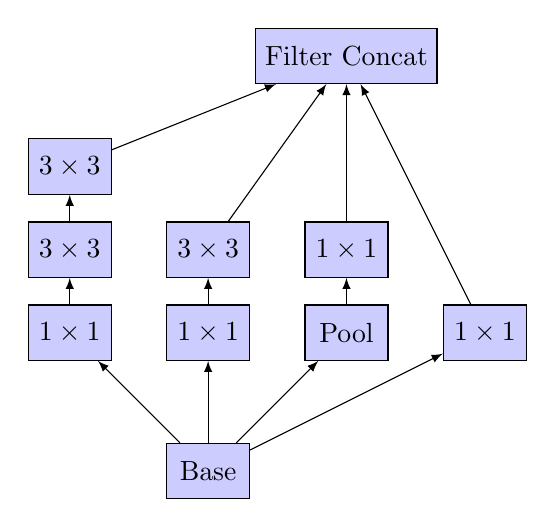
\begin{tikzpicture}[node distance=1.6cm]

    \node (concat) [block] {Filter Concat};

    \node (211) [block, below of=concat, node distance=7em] {$1\times1$};
    \node (233) [block, left of=211] {$3\times3$};
    \node (255) [block, left of=233] {$3\times3$};

    \node (333) [block, above of=255, node distance=3em] {$3\times3$};

    \node (pool) [block, below of=211, node distance=3em] {Pool};

    \node (1111) [block, left of=pool] {$1\times1$};
    \node (1112) [block, left of=1111] {$1\times1$};
    \node (1113) [block, right of=pool] {$1\times1$};

    \node (base) [block, below of=1111] {Base};

    
    \draw[arrow] (base) -- (1111);
    \draw[arrow] (base) -- (1112);
    \draw[arrow] (base) -- (pool);
    \draw[arrow] (base) -- (1113);

    \draw[arrow] (pool) -- (211);
    \draw[arrow] (1111) -- (233);
    \draw[arrow] (1112) -- (255);
    \draw[arrow] (1113) -- (concat);

    \draw[arrow] (255) -- (333);
    \draw[arrow] (333) -- (concat);
    \draw[arrow] (233) -- (concat);
    \draw[arrow] (211) -- (concat);

    

\end{tikzpicture}
    \captionof{figure}{Inception ModuleV2}
    \label{fig:incept_modul}
\end{minipage}




\subsubsection{Mobilenet}

\cite{howardMobileNetsEfficientConvolutional2017a}

Geringere Komplexität für Mobile oder embedded geräte, indem 
die normale Faltungsoperation mit der \textit{Depthwise Seperable 
Convolutions} ersetzt wird. 
Diese besteht aus einer \textit{Depthwise  
Convolutions}, welche die Faltunge auf 
die drei Farbchannel seperat anwendet udn einer 1times1
\textit{pointwise convolution}, welche die input channel combiniert. 

% \begin{figure}[H]
%     \centering
%     \includegraphics[width=0.5\textwidth]{DepthwiseSeperable.png}
%     \caption{DepthwiseSeperable}
%     \label{fig:mobilenet}
% \end{figure}
% %https://www.researchgate.net/publication/326727106/figure/fig1/AS:654646985113600@1533091412204/The-architecture-a-Standard-convolution-filters-b-Depthwise-convolutional-filters-c-1.png




In der zweiten version \cite{sandlerMobileNetV2InvertedResiduals2019} enthalten die 
Hauptbestandteile eine 1times1 conv mit relu, die 
3time3 depthwise gefolgt von einer weitere 1time1 ohne aktivierungsfunktion.

eine \textit{residual connection} unterstütz den gradientenfluss.

%https://towardsdatascience.com/mobilenetv2-inverted-residuals-and-linear-bottlenecks-8a4362f4ffd5
\begin{figure}[H]
    \centering
    \includegraphics[width=0.5\textwidth]{mobilenet_v2.png}
    \caption{MobilenetV2}
    \label{fig:mobilenetv2}
\end{figure}






%---------------- SUBSECTION: Obj Detection ----------------
\subsection{Objekterkennung}\label{subsec:objdet_det}

Neben der Information, was sich auf einem Bild befindet geht 
es bei der Objekt Erkennung auch darum herausfinden wo sich das 
Objekt auf dem Bild befindet.
Dafür wird die CNN Architektur so erweitert, dass dem 
Modell neben den Klassenlabels auch die Koordinaten 
der Bounding Boxen für das training mit übergeben werden.
Bounding Boxen umrahmen wie in Abbildung 
\ref{fig:class_vs_det} das Objekt auf dem Bild und 
werden meist über Regressionsverfahren 
angenähert.

Das gesammt Framework zur Objekterkennung 
verwendet dabei ein Basis CNN z.B. eines der in 
\ref{subsubsec:architectures} dargestellen. 

Das finden von Regionen, welche Objekte enthalten, 
kann dabei in einem seperaten, Netzwerk, welches 
Selective Search oder Vorschlagsgenerierer 
verwendet, stattfinden.



\vspace{1cm}
\begin{minipage}{0.5\textwidth}
    \centering
    Classification
\end{minipage}
\begin{minipage}{0.5\textwidth}
    \centering
    Detection
\end{minipage}
\begin{figure}[H]
    \centering
    \label{fig:class_vs_det}
    \includegraphics[width=0.8\textwidth]{classification_detection.jpeg}
    \caption{Unterschied: Classification - Detection}
\end{figure}




%------------------- SECTION: Hardware ----------------------
\section{Neural Compute Stick 2}\label{ncs2}

Da das Training und die Inferenz von Deep Learning Algorithmen
sehr rechenintensiv ist, werden entsprechen leistungsfähige 
Prozessoren benötigt. Dabei ist die Ausführung auf einer GPU 
(Graphical Processor Unit) meist effizienter als auf einer 
CPU (Central Processor Unit).

Anwendungen die auf eingebetteten Systemen laufe, wie etwa 
auf einem Raspberry Pi, kommen dabei schnell an ihre 
Grenzen.

Häufig werden daher die Bilddaten über eine Cloud zur 
verrechnung/inferenz an einen Leistungsstärkeren 
Rechner gesendet.

Sollen die Daten, wie dies beim Edge Computing der Fall ist, 
auf dem gerät direkt verarbeitet werden, gibt es speziell 
für die Inferenz von Deep Learing Algorithmen Ausgelegt 
Hardware, welche NN spezifische Berechnung besonders 
effizient durchführen kann.

Diese können entweder als eigenständiges \textit{System on Chip}
(SoC) System wie zb der \textit{Nvidia Jetson TX2} agieren oder 
zusammen mit einem Host, wie das bei dem in der Arbeit verwendeten 
Neural Compute Stick 2 der fall ist.

Dieser verwendet den Movidius Myriad X Vision Processing Unit (VPU)
welcher neben der Neural Compute Engine zur beschleunigten berechnung 
Neuronalen Netzen, einen Bildbeschleuniger, 16 SHAVE Prozessoren, 
Bildsignalprozessoren udn RISC CPU Core besitzt.
\cite{haussermannFunktionUndEffizienz}
\\[1cm]
\begin{minipage}{0.4\textwidth}
    \centering
    \label{fig:ncs2}
    \includegraphics[width=\textwidth]{ncs2_top.jpg}
    \captionof{figure}{ncsc2}
\end{minipage}
\begin{minipage}{0.6\textwidth}
    \centering
    \label{fig:myriad}
    \includegraphics[width=\textwidth]{myriad.png}
    \captionof{figure}{myriad}
\end{minipage}


\subsection{OpenVino Toolkit}

% doku:
% https://docs.openvinotoolkit.org/latest/_docs_IE_DG_Introduction.html
% diagramme:
% https://github.com/intel-iot-devkit/inference-tutorials-generic/tree/openvino_toolkit_2019_r1_0/car_detection_tutorial#tutorial-step-3-add-the-second-model-vehicle-attributes-detection
% https://github.com/intel-iot-devkit/inference-tutorials-generic/blob/openvino_toolkit_2019_r1_0/face_detection_tutorial/Readme.md


Um die Inferenz eines trainierten Deep Learing Modells auf dem
Neural Compute Stick ausführen zu können, wird das Toolkit 
\textit{OpenVino} verwendet.

Dieses ist eine Plattform zur Otimierung und Inferenz von 
CNN basierten Modellen auf unterschiedlicher Intel Hardware.





Dabei wird ein eigenes Dateiformat verwendet, die \textit{Intermediate 
Representation} (IR), welche die Struktur/Architektur des Modells 
in einer .xml Datei und die trainierten Parameter/Gewichte in 
einer Binary (.bin) datei abbildet.

Mit dem \textit{Model Optimizer} können Modelle der Frameworks 
TensorFlow, Caffe, ONNX, Kaldi, oder MXNET in das IR Format 
konvertiert werden.

Um diese dann auf die entsprechende Hardware zu laden und anwendbar 
zu machen, wird die auch in OpenVino enthaltene
\textit{InferenceEngeine} verwendet.

Diese bietet eine Api mit der aus der Anwendung heraus in den 
Programmiersprachen C++ oder Python auf die Funktionen der 
InferenceEngeine zugegriffen werden können.



\begin{figure}[H]
    \centering
    \def\svgwidth{0.8\textwidth}
    \input{Bilder/open_vino_workflow_neu.pdf_tex}
    \caption{OpenVino Workflow}
    \label{fig:openvinoflow}
\end{figure}


% \begin{figure}[H]
%     \centering
%     \includegraphics[width=0.8\textwidth]{./Bilder/open_vino_workflow_steps.png}
%     \caption{Workflow: OpenVino Toolkit}
%     \label{img:openvinoworkflow}
% \end{figure}

